
%%%%%%%%%%%%%%%%%%%%%%%%%%%%%%%%%%%%%%%%%%%%%%%%%%%%%%%%
% LaTex Template for proposals within the              %
% DFG Research Unit Program                            %         
%Planet Formation Witnesses and Probes: Transition Discs
% August 2016                                            %                           
%                                                      %
%%%%%%%%%%%%%%%%%%%%%%%%%%%%%%%%%%%%%%%%%%%%%%%%%%%%%%%%
%
% 
%
% This template may be used to prepare proposals in latex.
%
%
% The project description, including publication list, should be no more than 20 pages
% in length. It should be self-explanatory and not require reviewers to read the 
% literature that is quoted or enclosed.

\documentclass[10pt,fleqn,twoside]{article}

%%%%%%%%%%%%%%%%% GET THE STYLE STUFF %%%%%%%%%%%%%%%%%%%

%%%% USE ARIAL FONT %%%%%%%%%%%%%%%%%%%%%%%%%%%%%%%%%%%%%%%%%%%%%%%%%%%%%%
\usepackage{helvet}
\renewcommand\familydefault{phv}

%%%% INCLUDE NECESSARY PACKAGES %%%%%%%%%%%%%%%%%%%%%%%%%%%%%%%%%%%%%%%%%%
%\usepackage{babel}
\usepackage[UKenglish]{babel}
\usepackage{amsmath}
\usepackage{amssymb}
\usepackage{fancyhdr}
\usepackage{natbib}
\usepackage{ae,aecompl}
\usepackage{graphicx}
\usepackage{palatino}
\usepackage[T1]{fontenc}
\usepackage[right]{eurosym}
\usepackage{rotating}
\usepackage{epsf}
\usepackage{setspace}
\usepackage{xspace}
\usepackage{multicol}
\usepackage{siunitx}
%\usepackage{caption}

\usepackage{sfmath}

\usepackage[utf8]{inputenc}

% ========= hyperref & Colors & Links ===========
\usepackage[usenames,dvipsnames]{xcolor}
%\usepackage[breaklinks]{hyperref}
\usepackage{hyperref}
\addto\extrasUKenglish{%
\def\sectionautorefname{Section}%
\def\subsectionautorefname{Section}%
\def\subsubsectionautorefname{Section}%
\def\paragraphautorefname{Section}%
}
\usepackage[all]{hypcap} % fixes links to floats
\usepackage{aas_macros}  %
\setlength{\bibsep}{-0.5pt}

% ========= highlighting important parts of the proposal ===========
\definecolor{HighLight}{rgb}{0.9,0.3,0.0}
%\newenvironment{highlight}{\color{blue}\itshape}{\ignorespacesafterend}
%\newenvironment{highlight}{\color{RedOrange}\itshape}{\ignorespacesafterend}
%\newenvironment{highlight}{\color{RedOrange}\bfseries}{\ignorespacesafterend}
%\newenvironment{highlight}{\color{BrickRed}\bfseries\itshape}{\ignorespacesafterend}
%\newenvironment{highlight}{\color{BrickRed}\bfseries}{\ignorespacesafterend}
%\newenvironment{highlight}{\color{HighLight}\bfseries}{\ignorespacesafterend}
\newenvironment{highlight}{\color{HighLight}}{\ignorespacesafterend}
\newenvironment{missingenv}{\color{red}}{\ignorespacesafterend}

\definecolor{Emphasize}{rgb}{0.0,0.5,0.0}
\newenvironment{Emphasize}{\color{Emphasize}\itshape}{\ignorespacesafterend}


% strike through comments: to turn them off, uncomment the renewcommands below
\usepackage{soul}
\setstcolor{red}

% ========= Commands specially for the forschergruppe =========

\newcommand{\todo}[1]{\textcolor{red}{\bf #1}}
\newcommand\connect[1]{{\color{OliveGreen} #1}}

%%%% CAPTION LAYOUT %%%%%%%%%%%%%%%%%%%%%%%%%%%%%%%%%%%%%%%%%%%%%%%%%%%%%

\usepackage[font={small}]{caption}

%%%% PAGE LAYOUT %%%%%%%%%%%%%%%%%%%%%%%%%%%%%%%%%%%%%%%%%%%%%%%%%%%%%%%%%
\setlength{\textheight}{22cm}
\setlength{\topmargin}{-1.2cm}
\setlength{\textwidth}{15.6cm}
\setlength{\oddsidemargin}{0.0cm}
\setlength{\evensidemargin}{0.0cm}
\setlength{\mathindent}{1.5cm}
\setlength{\parindent}{0.0cm}
\setlength{\parskip}{0.08cm}

%%%% PAGE HEADER %%%%%%%%%%%%%%%%%%%%%%%%%%%%%%%%%%%%%%%%%%%%%%%%%%%%%%%%%%
\pagestyle{fancy}
\fancyhead[RE,RO]{}
\fancyfoot[RO]{\thepage}
\fancyfoot[LE]{\thepage}
\fancyfoot[CE,CO]{}

%%% FONTS FOR THE TITLE PAGE %%%%%%%%%%%%%%%%%%%%%%%%%%%%%%%%%%%%%%%%%%%%%%
\newfont{\tpfonta}{cmssbx10 scaled 1600}
\newfont{\tpfontb}{cmssbx10 scaled 3200}

%%%% COLOR DEFINITIONS %%%%%%%%%%%%%%%%%%%%%%%%%%%%%%%%%%%%
\definecolor{blue} {rgb} {0.25,0.25,0.75}

%%%% ADDITONAL EMPHASIS %%%%%%%%%%%%%%%%%%%%%%%%%%%%%%%%%%%
\newcommand{\cem}{\color{blue}}
\newcommand{\eem}{\sl\color{blue}}

%%%% BIBTEX PUNCTUATION %%%%%%%%%%%%%%%%%%%
\bibpunct{(}{)}{;}{a}{}{,} % to follow the A&A style

%%%% SET THE COLOR OF THE (SUB-) SECTION TITLES %%%%%%%%%%% 
\newcommand{\Tcol}{\color{blue}}

%%%% SET THE COLOR OF THE TITLE BOX BACKGROUND %%%%%%%%%%%%
\definecolor{Background}{rgb} {0.62,0.75,0.5}

%%%%%%%%%%%%%% REFERENCE SECTION NAME %%%%%%%%%%%%%%%%%%%%
\renewcommand\refname{\Tcol 9. Bibliography}

%%%%%%%%%%%%%% NICER PROJECT REFERENCES %%%%%%%%%%%%%%%%%%%

\newenvironment{literature}%
 {\begin{multicols}{2}\begin{scriptsize}\begin{list}{}{%
   \setlength{\topsep}{0em}%
   \setlength{\parskip}{0em}%
   \setlength{\parsep}{0em}%
   \setlength{\itemsep}{0em}%
   \setlength{\rightmargin}{0em}%
   \setlength{\leftmargin}{2em}%
   \setlength{\itemindent}{-2em}}}%
 {\end{list}\end{scriptsize}\end{multicols}}

%
% ...A compact itemize environment
%
\newenvironment{compactitemize}%
 {\begin{list}{$\bullet$}{%
   \setlength{\topsep}{0em}%
   \setlength{\parskip}{0em}%
   \setlength{\parsep}{0em}%
   \setlength{\itemsep}{0.0\baselineskip}%
   \setlength{\rightmargin}{0em}%
   \setlength{\leftmargin}{2.0em}%
   \setlength{\labelsep}{0.5em}%
   \setlength{\labelwidth}{1em}%
}}
 {\end{list}}

\newcounter{qcounter}
\newenvironment{compactenumerate}%
 {\begin{list}{\arabic{qcounter})~}{\usecounter{qcounter}%
   \setlength{\topsep}{0em}%
   \setlength{\parskip}{0em}%
   \setlength{\parsep}{0em}%
   \setlength{\itemsep}{0.0\baselineskip}%
   \setlength{\rightmargin}{0em}%
   \setlength{\leftmargin}{2.0em}%
   \setlength{\labelsep}{0.5em}%
   \setlength{\labelwidth}{1em}%
}}
 {\end{list}}

%%%% EXPLANATION FOR THE CONNECT COLOR %%%%%%%%%%% 
\newcommand{\footexplainconnect}{\footnote{The text highlighted in \connect{green} refers to the connection of this project to other projects of this Research Unit.}}
 
%%%%%%%%%%%%%%%%%% NICER REFERENCES %%%%%%%%%%%%%%%%%%%

%\usepackage[capitalise,nameinlink]{cleveref}
\newcommand{\cref}[1]{\autoref{#1}}

%%%%%%%%%%%%%%%%%% COLOR THE SECTION NUMBERS %%%%%%%%%%%%%%%%%

\makeatletter
\renewcommand\@seccntformat[1]{\color{blue} {\csname the#1\endcsname}\hspace{0.5em}}
\makeatother
\renewcommand\thesection{\arabic{section}.}
\renewcommand\thesubsection{\arabic{section}.\arabic{subsection}}

%%%%% color sections
\usepackage{sectsty}
\allsectionsfont{\color{blue}}


%%%% CHANGE THE APPEARANCE OF THE \PARAGRAPH COMMAND  %%%%%%%%%%%%%%%%%%%%%%%%%%%%%%%
\makeatletter
\renewcommand\paragraph{\@startsection{paragraph}{4}{\z@}%
            {-2.5ex\@plus -1ex \@minus -.25ex}%
            {1.25ex \@plus .25ex}%
            {\normalfont\normalsize\bfseries\Tcol}}
\makeatother
\setcounter{secnumdepth}{4}     % how many sectioning levels to assign numbers to
\setcounter{tocdepth}{4}        % how many sectioning levels to show in ToC

%%%%% set header

\renewcommand{\sectionmark}[1]{\markright{\color{black}#1}}

\newcommand{\caphighlight}[1]{{\bf #1}}



%%%%%%%%%%%%%%%%%%%%% TO DO MACROS %%%%%%%%%%%%%%%%%%%%%%

\let\todo\undefined   % Overwrite \todo command for this project
\usepackage[colorinlistoftodos,textwidth=2cm]{todonotes}
\newcommand{\missing}[1]{\textcolor{red}{\textbf{XXX #1 XXX}}}
\newcommand{\til}[1]{\todo[inline]{Til: #1}}
\newcommand{\kees}[1]{\todo[inline,color=LimeGreen]{Kees: #1}}

\newcommand{\tilchange}[2]{\textcolor{red}{(Til:)}\st{#1} \textcolor{red}{#2}}
\newcommand{\keeschange}[2]{\textcolor{red}{(Kees:)}\st{#1} \textcolor{red}{#2}}
\newcommand{\keesadd}[1]{\textcolor{red}{(Kees:)} \textcolor{red}{#1}}

\renewcommand{\tilchange}[2]{#2\xspace}
\renewcommand{\keeschange}[2]{#2\xspace}
\renewcommand{\keesadd}[1]{#1}

\newcommand{\twopoppy}{\texttt{twopoppy}\xspace}
\newcommand{\rebound}{\texttt{REBOUND}\xspace}
\newcommand{\pluto}{\texttt{PLUTO}\xspace}
\newcommand{\radmc}{\texttt{RADMC-3D}\xspace}

%%%%%%%%%%%%%%%%% DEFINE THE HEADER TEXT %%%%%%%%%%%%%%%%

\fancyhead[LO]{\fancyplain{}{\itshape Birnstiel \& Dullemond: RU
Transition Discs project C1}}
\fancyhead[RE]{\fancyplain{}{\itshape \rightmark}}
\fancyhead[LE]{}

%%%%%%%%%%%%%%%%%


\begin{document}


\newpage

%%%% PROJECT DESCRIPTION STARTS HERE %%%%%%%%%%%%%%%%%%%%%%%%%%%%%%%%%%%

\setcounter{page}{1}

\centerline{\huge\bf\Tcol
%
%
%
%
%%%%  Please edit
%
 Project C1:}
\vspace{1em}

\centerline{\LARGE\bf\Tcol Trapping the dust:}\vspace{0.3em}
\centerline{\LARGE\bf\Tcol  Planet formation `hotspots' in TDs}

%
%%%%
%
%
%
%
\vskip1.0cm

%%%%  Please edit

\noindent{\bf Authors:}\\
\begin{tabular}{ll}
{\textsf{PIs:}}            & T.~Birnstiel (LMU) \\
                           & C.P.~Dullemond (U. Heidelberg)\\
{\textsf{Co-I:}}           & W. Kley (U. Tübingen) \\
{\textsf{Collaborations:}} & van Dishoeck (Leiden/MPE) \\

\end{tabular}

%%%%  Please edit

\vspace{1em}
\noindent{\bf Requested positions: 1 PhD student} \\

\vspace{1em}
\noindent{\bf Abstract:}\\
Based on our current understanding of the physics of planet formation,
several processes seemingly prevent or stall the growth towards larger
bodies:
(1) collisional growth is inefficient above $\sim$meter-sizes,
(2) fast radial migration removes solid particles on very short time
scales,
(3) large particles need to locally accumulate above the canonical
dust-to-gas ratio in order to trigger gravoturbulent formation of
planetesimals, and
(4) radial migration of pebble-sized particles renders the accretional
growth of planetesimals inefficient.
Observations of transition disks suggest that they provide the
environments, where all of these issues can be solved: trapping and
growth of solid particles in the pressure bumps of transition disks
can provide the large enough particles at high enough densities to
trigger gravoturbulent planetesimal formation. Additionally, the
trapped particles are not drifting away, meaning they can be
efficiently accreted onto the growing planetesimals. It is the goal of
this proposal to investigate the trapping, planetesimal formation, and
planetesimal growth processes in these apparent `planet formation
hotspots' in transition disks.

%Pebbles drifting through a swarm of planetesimals, however, are not
%efficiently swept up due to the high speed at which the pebbles cross
% the planetesimal orbits.

\section{State of the art and preliminary work}

\subsection*{State of the art: Transition Disks and Planet Formation}

With over to 3000 detected planets, it is striking that we still do
not understand how planets form. Their building blocks, the
\textit{planetesimals} form in gas disks around young stars, where
colliding dust grains form ever-larger aggregates. But this growth is
not without limits: larger particles quickly drift towards the star
and collide at speeds that shatter them to pieces, long before gravity
can bind them together. The mechanisms involved in the assembly and
transport of these building blocks remain some of the biggest
mysteries of planet formation.

Over the last couple of decades, observations of protoplanetary disks
have revolutionized the field of planet formation. This started with
surveys of disks \citep[see the review of][]{2011ARA&A..49...67W} and
continued with ever better imaging campaigns \citep[e.g.,][and many
others]{2007ApJ...659..705A,2009ApJ...704..496B}.
Early imaging results of \citet{2008ApJ...675L.109B} and
\citet{2009ApJ...704..496B} revealed for the first time depleted inner
cavities in disks that were previously just suspected from the
spectral energy distributions. These disks with holes were initially
thought to be in the process of transitioning from a gas rich disk
to a gas poor disk \cite[e.g.,][]{2001MNRAS.328..485C} and thus termed
\textit{transition disks} \citep[see][and references
therein]{2014prpl.conf..497E,2014prpl.conf..475A}.

As statistics and theoretical models improved, it became clear that
this cannot be the full story: some of the inner holes were found to
be clearly too large and the disk accreting too vigorously to be
explainable by current models of photoevaporation
\citep[i.e.\ Type 2 TDs,][]{2010MNRAS.401.1415O,2011MNRAS.412...13O}.
Other explanations were discussed, such as particle growth
\citep{2005A&A...434..971D,2005ApJ...625..414T,2012A&A...544A..79B} or
gap opening by planets
\citep{2004A&A...425L...9P,2006A&A...453.1129P,2006MNRAS.373.1619R,
2012A&A...545A..81P,2012ApJ...755....6Z}. Most of these models have in
common that some mechanism (e.g., photoevaporation,
planet-disk-interaction, or others) produce a pressure maximum.
Solid particles that have collisionally grown to macroscopic sizes
experience fast radial migration towards higher pressure
\citep{1972fpp..conf..211W,1977MNRAS.180...57W,1986Icar...67..375N}.
Already \citet{1972fpp..conf..211W} suggested that particles moving
due to this effect can become \textit{trapped} in a pressure maximum,
as depicted in \autoref{fig:whipple} taken from his paper. One of
the first images of such a ring-like transition disk, from
\cite{2009ApJ...704..496B} is shown in \autoref{fig:brown}.


\begin{figure}
\centering
\begin{minipage}[b]{.47\textwidth}
  \centering
  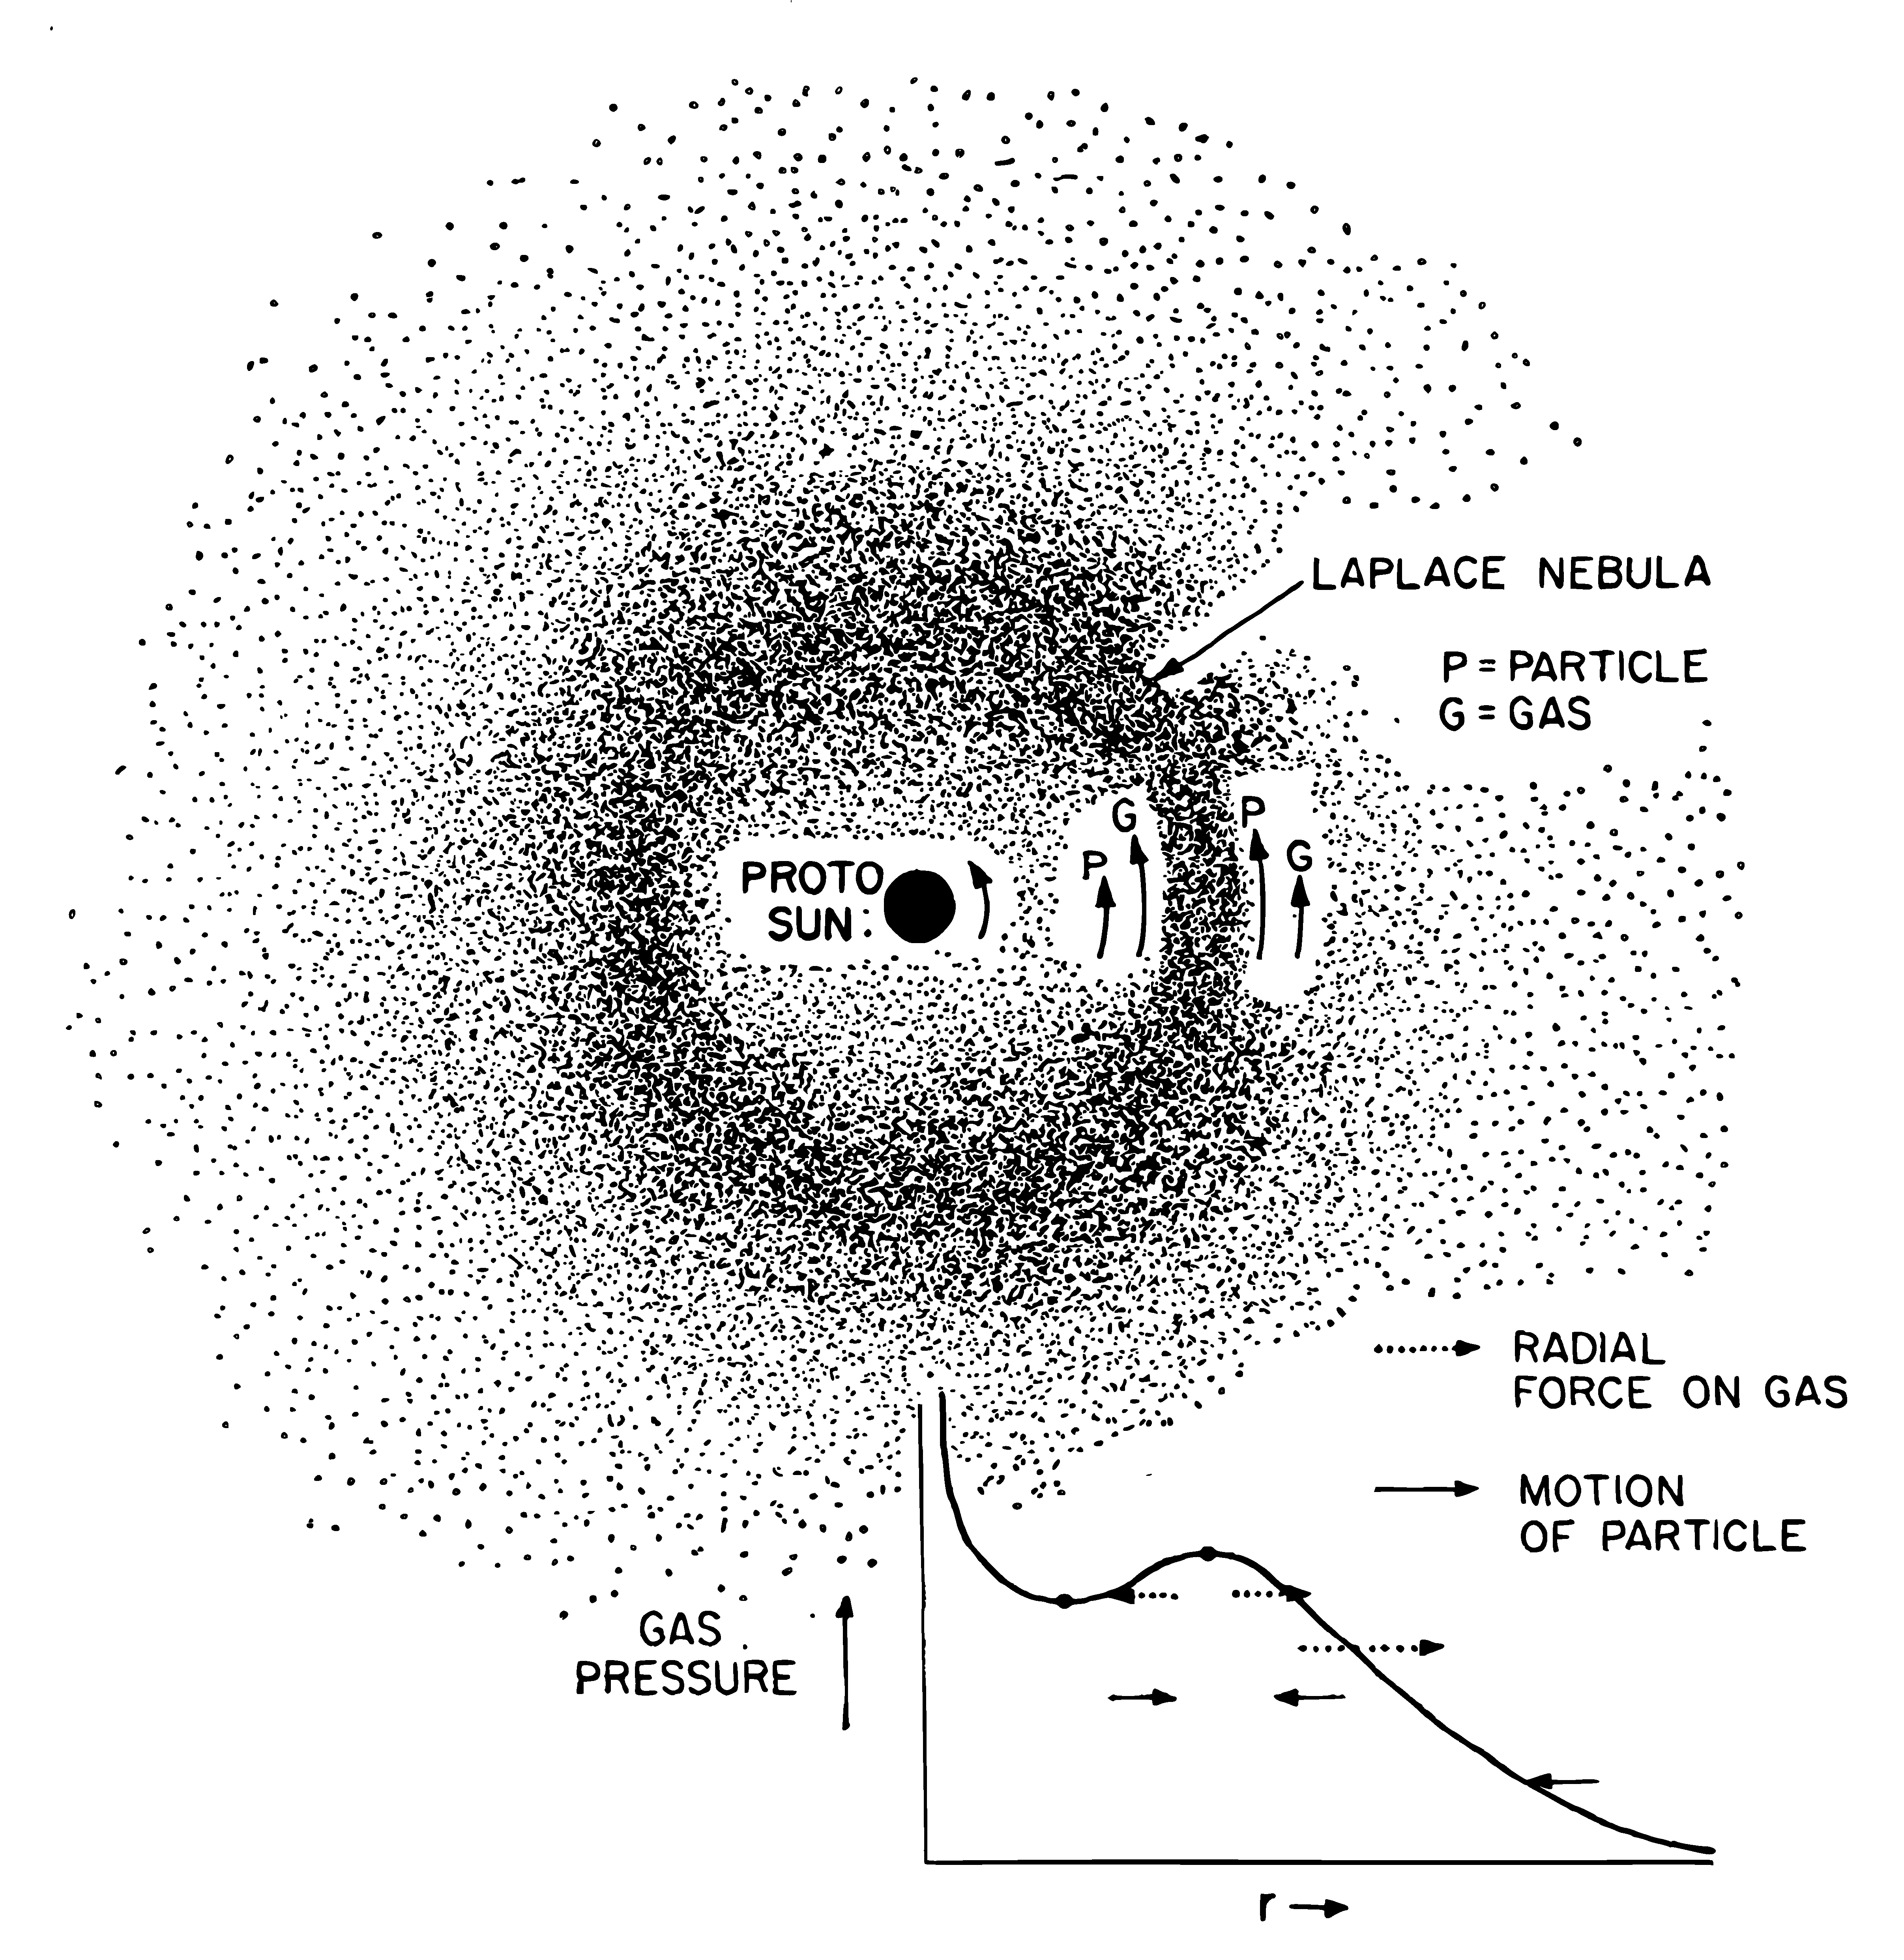
\includegraphics[width=\linewidth]{C1fig/Whipple1972-Fig1_traced}
  \captionof{figure}{Accumulation of solid particles in pressure
  bumps. Taken from \citet{1972fpp..conf..211W}.\newline\newline}
  \label{fig:whipple}
\end{minipage}%
\hspace{0.05\textwidth}
\begin{minipage}[b]{.47\textwidth}
  \centering
  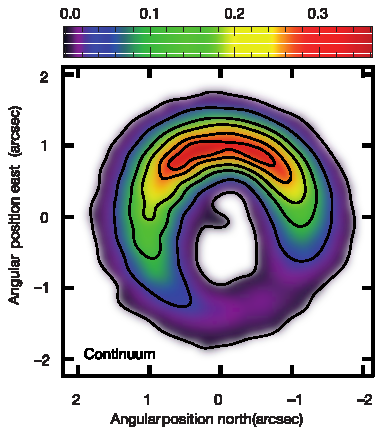
\includegraphics[width=\linewidth]{C1fig/casassus2}
  \captionof{figure}{Early imaging of ring-like
  accumulations of dust in the transition disk SR 21N. Taken from
  \citet{2009ApJ...704..496B}. Units are in \si{Jy/beam}.
  \missing{update caption and all references}}
  \label{fig:brown}
\end{minipage}
\end{figure}

Statistical analysis of the occurrence rates and properties of
transition disks suggested that there are two families of transition
disks: a family of small accretion rate / small hole sizes / small
disk mass and another family of larger hole sizes accompanied by
larger disk masses and higher accretion rates
\citep{2012MNRAS.426L..96O}. While the possibly diverse
\textit{origins} of transition disks are still obscure, the
observations at face value already show us something even more
interesting: large fractions of the solid contents of the disks can be
contained near the inner edge of the outer disk.
These cavity edges should therefore be prime regions for the formation
of planetesimals or even planets. As such, transition disks are not
only interesting probes of disk evolution or disk dispersal, but may
allow us to study in detail what role pressure bumps are playing in
the formation of planets.

In 2013, we proposed  that the dust trapped in a slightly lopsided gas
disk (i.e.\ an azimuthal pressure bump) can become extremely
concentrated in that azimuthal over-density
\citep[see][]{2013A&A...550L...8B}. In the same year, we were part of
a team that published and analyzed ALMA observations of the disk Oph
IRS 48 that showed such an extreme asymmetry, as predicted by the
models \citep[see][]{2013Sci...340.1199V}. It is widely accepted that
the dust accumulations in pressure bumps (whatever their formation
mechanism may be) are prime regions -- \textit{hot spots} -- of planet
formation: accumulation of particles in pressure bumps
\citep[e.g.,][]{2007ApJ...664L..55K} prevents them from drifting away
and shortens the growth time scales of dust particles allowing further
growth \citep{2008A&A...487L...1B}. Accumulation of these particles
can trigger the streaming instability which needs particle
accumulations and particles of the right sizes to operate
\citep{2005ApJ...620..459Y,2007Natur.448.1022J}.
Vortices further support the accumulation to critical densities
\citep{1995A&A...295L...1B,1997Icar..128..213K,2015ApJ...804...35R} or
even the direct formation of earth sized objects
\citep{2009A&A...493.1125L}.

Another revolution in the field of planet formation came not from the
observational, but from the theoretical side. It was shown that small
particles can very effectively be accreted onto planetesimals under
the right conditions when gas drag effects increase the effective
cross section of the accreting body
\citep{2010A&A...520A..43O,2012A&A...544A..32L}. It has turned out
that this process -- termed \textit{pebble accretion} -- can be
dominant over the late-stage oligarchic growth and giant impact growth
if the flow of pebbles can be controlled \citep{2015Natur.524..322L},
although the exact ratio of mass that is accreted via planetesimals
and via smaller particles is still under investigation, as is the
efficiency of the process
\citep[see][]{2014A&A...572A..72G,2016A&A...586A..66V,2016arXiv160708250O}.
But there is a problem with this and that is the fact that
planetesimals seem to be formed big \citep[][Klahr et al., submitted
to Nature]{2009Icar..204..558M} with sizes around \SI{100}{km}. This
happens to be the size at which pebble accretion onto the
planetesimals is particularly inefficient \citep{2016A&A...586A..66V}.

\begin{highlight}
In other words: planetesimals likely form 100-km-sized bodies, but
only if over-densities of pebble sized objects are present. Further
growth of planetesimals of this size is inefficient unless there is a
large reservoir of particles of the right sizes available to be
accreted. Pressure bumps, such as the ones observed in transition
disks provide the right conditions to solve both of these problems.
\end{highlight}

Several authors have already investigated the dynamics of particles in
and around planetary gaps in disks. Some of the recent work includes
\citet{2004A&A...425L...9P,2006A&A...453.1129P},
\citet{2006MNRAS.373.1619R}, \citet{2009A&A...493.1125L},
\citet{2012ApJ...755....6Z}, \citet{2012A&A...547A..58G},
\citet{2013A&A...553L...3A}, or \citet{2015A&A...584A.110P}, to name
just a few. Most of these works have in common, that they follow only
small particles that are not growing in size and they do not follow
planetesimals or their growth at the same time. These works are mainly
aimed at explaining the observed properties of transition disks, but
surprisingly little work has been done to understand how transition
disks -- or pressure bumps in general -- regulate the formation of
planets or planetesimals. Some authors \citep[e.g.,][and following
papers in that series]{2014ApJ...780...53C} have pointed out how
pressure bumps and planet formation can trigger each other, leading to
a inside-out planet formation scenario. This is a promising scenario
to explain for example the systems with tightly packed inner planets
discovered with the Kepler Mission \citep{2012ApJ...761...92F}.
However the details of what happens to the dust and larger bodies in
the pressure bump has not been subject of a dedicated study yet.

With this proposal, we want to build on our expertise on dust
evolution and particle trapping in protoplanetary disks to study the
formation of planetesimals in pressure bumps, their further
evolution due to dynamics, interaction with the gas disk,
interaction with other planetesimals, and growth due to accretion of
pebbles.

\begin{highlight}
The goal of this proposal is to understand how planetesimal
and planet formation proceeds in pressure bumps and to find out
if transition disks are indeed the hot-spots of planet formation that
we think they are.
\end{highlight}

\subsection*{Preliminary Work}

Both PIs have extensive experience in the physics of particle growth
and dynamics of dust particles \citep[e..g][see
\citealp{2016SSRv..tmp...32B} for a recent
review]{2005A&A...434..971D, 2008A&A...480..859B, 2008A&A...489..931Z,
2010A&A...513A..79B, 2012A&A...539A.148B, 2014A&A...572A..78D} as well
as in disk structure and evolution \citep[e.g.,][and many
others]{2001ApJ...560..957D, 2002A&A...389..464D, 2004A&A...417..159D,
2010ARA&A..48..205D,2015ApJ...813L..14B}. Furthermore, C.P. Dullemond
has been supervising or contributing to several works on
planet-disk-interaction, vortex-formation, and
planet-vortex-interaction
\citep{2012MNRAS.419.1701R,2013A&A...553L...3A,2014A&A...572A..61A}.

More recently, a collaboration between the PIs of this proposal and
the group of Dr.\ Hui Li at Los Alamos National Labs (LANL), USA has
been established. Dr.\ Hui Li has been pioneering the field of
vortex formation in the context of protoplanetary disks
\citep{2001ApJ...551..874L,2000ApJ...533.1023L}. Furthermore, the LANL
group has extensive experience in hydrodynamical modeling and more
recently in modeling dust dynamics via tracer fluids
\citep[e.g.,][]{2014ApJ...795L..39F,2016ApJ...818...76J}.

Dr.\ T.\ Birnstiel has worked on two-dimensional models of dust
evolution, treating particle growth, fragmentation, turbulent mixing
and vertical settling. Preliminary results of this are shown in
\autoref{fig:2dplot} in the left column. Similar work on this, but in
the radial/azimuthal dimensions is ongoing as part of the collaboration
with the LANL group. The right hand side panels in \autoref{fig:2dplot}
show a proof of concept simulation where gas dynamics as well as dust
dynamics of around 100 different particle sizes are taken into
account. Subroutines for simulating particle growth and fragmentation
have been developed and are currently being tested.

\begin{highlight}
To continue this work on particle growth in two dimensions as well as
work on other related topics, Dr.\ T.\ Birnstiel has recently been
awarded an \textit{ERC Starting Grant} which will start in March 2017
at the LMU Munich. By becoming part of this Research Unit, Dr.\ 
Birnstiel will share the progress and the resulting data with the
research group wherever other projects of the Research Unit profit
from it. This includes, but is not limited to, the dust density
distribution $\rho_\mathrm{dust}(r,z,a)$ as function of distance to
the star $r$, height above the mid-plane $z$, and particle size $a$
and similar results from the radial/azimuthal models.
\end{highlight}

\begin{figure}
\centering
  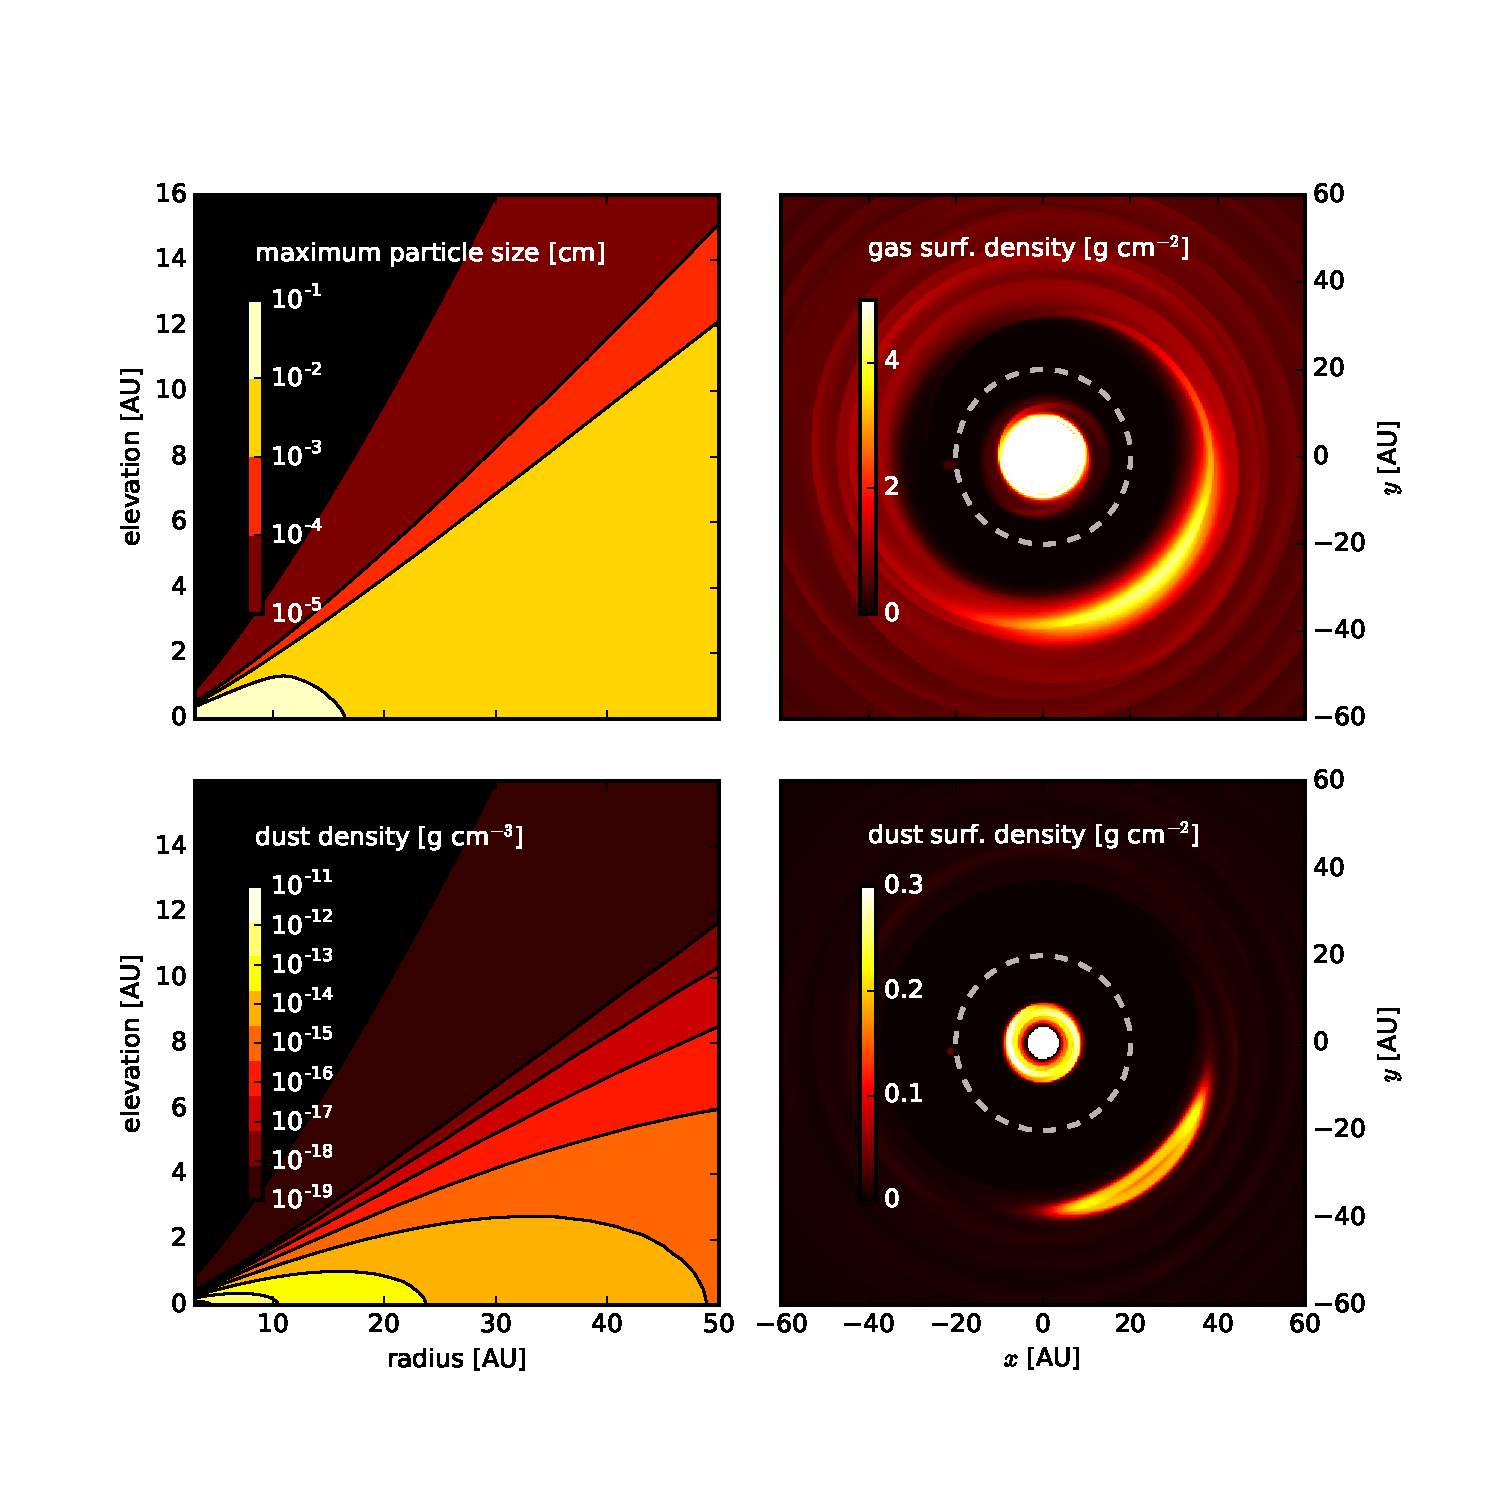
\includegraphics[width=\linewidth]{C1fig/2dplot_new}
  \captionof{figure}{Proof-of-concept models for 2D dust
  evolution simulations. The panels to the \caphighlight{left} show the
  radial/vertical distribution of solids (\caphighlight{top}) and maximum particle
  sizes (\caphighlight{bottom}) where both coagulation and vertical transport
  processes are treated at each point of a 2D grid. The panels on the
  \caphighlight{right} show radial/azimuthal results of the LA-COMPASS code (in
  normalized code units, resolution of 1024$\times$1536) that is now
  able to treat 100s of particle sizes and their size evolution. The
  \caphighlight{top} panel shows the distribution of gas surface density where a
  planet, orbiting on the dashed line, carves a gap and forms a
  pressure bump outside of its orbit. The pressure bump becomes Rossby
  unstable and the resulting vortex efficiently traps larger
  particles. The distribution of 0.09 mm sized particles is shown in
  the \caphighlight{lower right}.\missing{Fix lower left color bar}}
  \label{fig:2dplot}
\end{figure}

\subsection{Project-related publications}

% Please list your own publications related to the proposed project, 
% adhering to the rules of the DFG guidelines 1.91. In brief, please note: 
% - Up to 10 publications
% - The work must be published or accepted.
% - Publications on astro-ph (arXive, SPIRES or articles with a DOI) count as published. 
% - Any work that is only in the status ``accepted'' MUST be attached to the proposal
%    together with the acceptance letter.
% - All publications in this section CAN be attached to the proposal. Please limit these
%    attachments to a minimum and please note that the reviewers may not read the attachments -
%    the proposal has to speak for itself.
% - The number of allowed publications refers to the sum of the publications listed
%    in ``1.1.1 Articles published or officially accepted by publication outlets...'' and 
%    in ``1.1.2 Other publications''. Publications which only exist on public repositories 
%    belong into the category ``Other Publications''.
\begin{literature}
\item \textbf{Birnstiel, T.}, \textbf{Dullemond, C.P.} \& Brauer, F.,
  \textit{Gas and dust evolution in protoplanetary disks}, 2010, A\&A
  513, 79. In this paper we present the basic code for the evolution
  of the disk and the dust.
  The latter follows the dust coagulation, fragmentation, settling and
  radial drift of the dust.
\item S\'andor, Z., Lyra, W., \textbf{Dullemond, C.P.}, {\em Formation
  of PlanetaryCores at Type I Migration Traps}, 2011, ApJ, 728, L9.
  Here we performed detailed N-body calculations of multi-planet
  systems with migration torques. This experience helps us with
  determining the dynamics of pebbles as they approach the planet. The
  migration torque is then replaced by gas friction.
\item \textbf{Birnstiel, T.}, Klahr, H. \& Ercolano, B.: \textit{A
  simple model for the evolution of the dust population in
  protoplanetary disks}, 2012, A\&A 539, 148. In this model the flow
  of pebbles from the outer disk regions into the inner planet forming
  disk regions is studied, and an easy to use model derived.
\item \textbf{Birnstiel, T.}, Andrews S.M., Ercolano B. \textit{Can
  grain growth explain transition disks?}, 2012, A\&A, 544, A79. We
  showed that particle coagulation in itself can successfully create
  observed transition disk signatures at infrared wavelengths, but
  fails to produce the central cavities at (sub-)millimeter
  wavelengths.
\item Pinilla P., Benisty M., \textbf{Birnstiel, T.} \textit{Ring
  shaped dust accumulation in transition disks}, 2012, A\&A, 545, A81.
  We presented the first model that explained transition disks trough
  a combination of particle growth and transport processes and the
  pressure trap created by a giant planet.
\item Ataiee, S., Pinilla, P., Zsom, A., \textbf{Dullemond, C. P.},
  Dominik, C., Ghanbari, J. \textit{Asymmetric transition disks:
  Vorticity or eccentricity?}, 2013, A\&A, 553, L3. We demonstrated
  how asymmetries in dust disks can be produced by vortices or by disk
  eccentricity and how these methods cause very different dust density
  contrasts. 
\item van der Marel N., van Dishoeck E.F., Bruderer S.,
  \textbf{Birnstiel, T.}, Pinilla P., \textbf{Dullemond, C.P.}, et
  al.: \textit{A Major Asymmetric Dust Trap in a Transition Disk}
  2013, Science, 340(6), 1199. First observation of an extremely
  lopsided dust disk that was interpreted as trapping of solids in a
  vortex-like structure.
\item Ataiee, S., \textbf{Dullemond, C. P.}; Kley, W., Regály, Zs.,
  Meheut, H. \textit{Planet-vortex interaction: How a vortex can
  shepherd a planetary embryo}, 2014, A\&A, 572, A61. We studied how a
  vortex interacts gravitationally with a migrating planet or with a
  planet that is created inside the vortex.
\item Pinilla, P., Klarmann, L., \textbf{Birnstiel, T.}, Benisty, M.,
  Dominik, C., \textbf{Dullemond, C.P.} {\em A tunnel and a traffic
  jam: How transition disks maintain a detectable warm dust component
  despite the presence of a large planet-carved gap}, 2016, A\&A 585,
  A35. Here the dust coagulation and trapping model is extended to
  explain the shape of pre-transitional disks via incomplete trapping,
  coagulation and fragmentation near the water ice line.
\end{literature}

% \subsubsection{ 
% Articles published or officially accepted by publication outlets with scientific quality assurance;
% book publications}
% 
% \missing{Text}
% 
% \subsubsection{ Other publications}
% 
% None
% 
% \subsubsection{Patents}
% 
% \paragraph{Pending}
% 
% None
% 
% \paragraph{Issued}
% 
% None

\section{Objectives and work programme}


\subsection{Anticipated total duration of the project}

36 Months

\subsection{Objectives}

The goal of this project is to investigate the growth and dynamics of
planetesimals and of forming planets in pressure bumps of transition
disks. The scientific questions we want to answer are:

\begin{itemize}
  \item How effectively can planetesimals be formed in pressure bumps?
  \item What properties of the pressure bumps are compatible with
  observational properties of protoplanetary disks?
  How effective can planet(esimal) formation be in transition disks?
  At what efficiency will it start violating observational properties
  of observed disks?
  \item Is growth via mutual collisions or accretion of pebble sized
  dust the dominant mode of planetesimal growth?
  \item What role does the dynamical evolution play -- how large can
  planetesimals grow before their dynamics either leads to destruction
  or causes them to leave their birth places? Related: how will a
  newly formed planet in the bump move around the remaining pebbles?
  Will there be observational signals of such a planet in the shape of
  the dust concentration and its polarized signature \citep[see,
  e.g.,][]{2016ApJ...831L..12K}?
  \item How does the origin of the pressure bump (e.g.\ viscosity
  bump, photoevaporation, or planet) affect these scenarios?
  \item How does the situation change with various parameters such as
  the extent of the pressure bump, the turbulence strengths or
  in particular with vortices in case the pressure bump becomes
  Rossby wave unstable?
\end{itemize}

\subsection{Work programme including proposed research methods}

\subsubsection{Research Methodology}

In this project, we will couple the evolution of small solid particles
via recipes of gravoturbulent planetesimal formation to the growth and
dynamical evolution of planetesimals. To do this, we will will employ
two different methodologies: first, we will use simplified gas disk
structure models (i.e.\ hydrostatic disks). Therefore, we will be able
to concentrate on the dust processes and the planetesimal formation
and dynamical evolution processes in more detail. This methodology
will encompass phase I and II (cf. \autoref{sec:phaseI} and
\autoref{sec:phaseII}). The second approach in phase III (cf.
\autoref{sec:phaseIII}) will include detailed hydrodynamical processes
but therefore necessarily simplifying other aspects such as the dust
evolution. This simplification, however, will be based on the results
of phase I and II (and the ERC project of Dr.\ Birnstiel) and will thus
\textit{not} be based on ad-hoc assumptions.

\subsubsection{Research Tools and Inputs}
For this project, we will be using the following tools:

\begin{itemize}
  \item A dust evolution code, either the open-source code \twopoppy
  \citep{2012A&A...539A.148B}, described below, or if needed, the
  gas+dust disk evolution code of \citet{2010A&A...513A..79B}.
  \item A N-body integrator. For this we will the open-source code
  \rebound, which offers a wide variety of integration schemes and
  flexible options to include additional forces or add/remove
  particles.
  \item A disk hydrodynamical code with Lagrangian particles. The
  foundation of this will be the custom version of the \pluto code
  from \citep{2015A&A...584A.110P}. We will use this code or future
  versions of it in phase III (\autoref{sec:phaseIII}) and implement
  the growth processes developed in phase I and phase II.
  \item For comparison with dust continuum observations, we will
  employ the 3D monte carlo radiative transfer code \radmc that was
  developed by the co-PI Prof.\ Dullemond. Scripts to directly run the
  \radmc dust radiative transfer calculation with the input from the
  dust evolution code of co-PI Dr.\ Birnstiel are available. These
  include opacity calculations as well as hydrostatic equilibrium
  iteration with dust-settling-mixing solutions for each particle
  size.
\end{itemize}

\subsubsection{Research Plan}

\paragraph{Phase I: Planetesimal formation and simple gas
structures}
\label{sec:phaseI}

The student will begin by getting acquainted with the astrophysics of
disks and planet formation on the one side and and with the numerical
methods on the other side. The initial setup will be an axisymmetric
pressure bump profile. For this, we will start with a parametrized,
stationary pressure bump in our one dimensional dust/gas code
\twopoppy\footnote{\url{http://birnstiel.github.io/two-pop-py/}}
\citep{2012A&A...539A.148B}. Further gradual improvements will include
an $\alpha$-disk evolution (already implemented in the code) where the
pressure bump forms due to parametrized variations in the
$\alpha$-viscosity \citep{2007ApJ...664L..55K}. This will allow us to
look at time-dependent trapping processes, e.g.\ for pressure bumps
with a finite life time. If necessary, the viscous radial evolution of
the gas density could also be treated using 1D hydrodynamics to
account for deviations in the rotation profile near the bump.

The student will then implement a subroutine that converts small dust
particles to planetesimals whenever the right conditions are
fulfilled. Similar methods have already been used by the PIs
\citep[][and Klahr, Birnstiel, Lenz, in prep.]{2014A&A...572A..78D}.
We will use Eq.~12 of \citet{2014A&A...572A..78D}, which is a fit to
detailed numerical results of \citet{2010ApJ...722.1437B} consistent
with other works on planetesimal formation in the context of the
streaming instability \citep[e.g.,][]{2009ApJ...704L..75J}. Based on
the local metallicity and the resulting planetesimal formation
efficiency, dust mass will be removed via a sink term and the
resulting mass in planetesimals will be tracked (without further
evolution of the planetesimals at this point). The particle size
distribution can be reconstructed using the methods published in
\citet{2015ApJ...813L..14B}. Should we find that the accuracy of this
method is not sufficient (i.e.\ if the results are very sensitive to
one of the approximations done here), then we could switch to an
implementation of the code presented in \citet{2010A&A...513A..79B}.
This will be more accurate and more detailed, but also significantly
slower but not prohibitively slow as the N-body dynamics of the later
stages of the project will be more limiting. The calculations outlined
above will lay the foundation of the next parts of the proposed
research plan:

\begin{itemize}
  \item They provide the accretion rate of dust particles into
  the pressure bump.
  \item They provide the size distribution of the particles entering
  the pressure bump.
  \item The subroutine will calculate how much of the available dust
  is transformed into planetesimals.
\end{itemize}

Using the code at this stage, we will already be able to publish a
first paper describing the methods and our results on planetesimal
formation rates comparing to previous works in this direction
\citep[e.g.,][]{2014A&A...572A..78D, 2016A&A...586A..20K}. Some
mechanisms creating pressure bumps have a finite life time, such as
zonal flows, or pressure bumps at the edges of dead zones. Using bumps
of finite life time will allow us to investigate the efficiency of
particle trapping in time-dependent pressure maxima and their possible
relation to Type I transition disks, which is a significant
improvement over previous works such as \citet{2012A&A...538A.114P}
and \citet{2013A&A...554A..95P}. By linking this to existing
millimeter wave radio-surveys (e.g.,
\citealp{2016ApJ...831..125P} and references therein as well as
previous surveys such as \citealp{2010A&A...521A..66R}) we will be
able to test which bump amplitudes, bump sizes, and life times are
producing results consistent with (1) dust continuum observations and
(2) dust disk life times. This way, we will be able to exclude or
constrain some of the theoretically proposed mechanisms, such as zonal
flows \citep[e.g.,][]{2009ApJ...697.1269J, 2013ApJ...763..117D,
2014ApJ...796...31B}.

\paragraph{Phase II: N-Body dynamics and planetesimal evolution}
\label{sec:phaseII}

In Phase I, planetesimals are formed at a given rate based on
calculations of the dust evolution code, however the forming
planetesimals are just kept on record and are not evolving further.
Phase II of this proposal aims at improving upon this. At the
beginning of the project, we will use the modular, and easy to use
N-body integrator
\rebound\footnote{\url{http://github.com/hannorein/rebound}}
\citep{2012A&A...537A.128R}. The fact that both \twopoppy and \rebound
have python interfaces simplifies linking them: based on the
planetesimal formation rates and the gas and dust surface densities
from \twopoppy, particles (planetesimals) can be created in \rebound.
Initially, planetesimals might be tracked individually, but as their
number increases, we will likely need to switch to a super-particle
approach, where one individual particle in the code represents a
larger number of physical planetesimals.

The gas and dust density distribution is still assumed to be
axisymmetric at this point, but an analytical vertical distribution of
the density will be assumed to create a 3D density distribution: the
gas will be assumed to be in hydrostatic equilibrium, while the dust
will be in a mixing-settling equilibrium \citep{2009A&A...496..597F}.

At this point of the proposal, there are two parallel directions in
which the simulation tools will be improved, linking to two different
scientific directions: one focuses on more detailed gas dynamics that
has links to project \textbf{C2} and will be discussed below in
\autoref{sec:phaseIII}. In this phase II of the research plan
we will focus on the N-body treatment of the planetesimals and related science
questions (to clarify: pebbles are treated as a fluid).

Based on the dust particle sizes and the 3D distribution of dust and
gas developed above, we can calculate the accretion rate of pebbles
onto the planetesimals. This will use the prescriptions of
\citet{2010A&A...520A..43O}, \citet{2016A&A...586A..66V} and related
works. Based on these rates, calculated/updated at appropriate time
intervals, the mass of the N-body particles (in the \rebound code)
will be increased and the total mass of accreted dust particles will
be removed as sink terms in the \twopoppy code. This way the evolution
of planetesimals and of the dust distribution affect each other:

Planetesimals (1) form based on the local metallicity and (2) grow via
pebble accretion of dust particles of the right sizes. Dust, on the
other hand, is removed by both of these effects, but possibly and to a
smaller extend replenished by fragments. If these dust removal
processes are efficient no further planetesimals will be formed since
the metallicity in the bump will be kept below critical values.
As another consequence, the reduction in dust mass might also reduce
the particle sizes which further minimizes the amount of particles
contributing to planetesimal formation. This latter effect will,
however also decrease the efficiency at which the dust is accreted
onto the planetesimal.
Based on this, various outcomes of the early stages of planet
formation could be imagined:
\begin{itemize}
  \item Planetesimals form but then prevent further planetesimal
  formation, instead efficiently growing via pebble accretion (and
  possibly oligarchic growth at the same time).
  \item  Planetesimal formation may be too efficient: many
  planetesimals form leaving little amounts of dust to be accreted
  onto the planetesimals. At this point dynamical and collisional
  evolution of planetesimals may become the dominant driving force.
\end{itemize}

As this shows, it will be extremely interesting to see how the
formation of larger bodies proceeds in the hot-spots of planet
formation in transition disks. This project so far already
incorporates aspects of gas dynamics, collisional evolution and
dynamics of small dust particles and N-body dynamics, a seemingly
challenging combination. However, we would like to point out that the
methods and codes we use for this are well established: the \rebound
code for example allows scientifically relevant calculation with only
a few lines of code. It offers a wide variety of well tested and well
documented integrators and a simple object-oriented approach to handle
additional forces or close encounters. The \twopoppy code as well can
be run with only a hand full of lines of code and well reproduces the
results of complicated coagulation codes. Combining these codes offers
a student interesting quick successes but still the opportunity to
gradually learn the numerical methods and also the physical processes
used and assumed ``under the hood'' of these codes.

At the end of this phase II of the project, we anticipate at least one
more publication that describes the numerical setup and explains the
findings of a parameter study. With this study, we will be able to
calculate planetesimal formation rates under various trapping
conditions and study how the general outcome but also the detailed
size distribution of planetesimals varies with disk parameters. We
will also test under which conditions an analytical treatment of the
involved effects, based on rate equations, can be found. Follow up
studies can include improved collision models, effects of turbulence
on the planetesimal distribution and many other effects.

\paragraph{Phase III: Breaking the Symmetry}
\label{sec:phaseIII}

So far the distribution of both dust and gas has been assumed to be
symmetric. As observations show us, this is indeed the case in many
transition disks, as well as in disks with small scale axisymmetric
structure, such as HL Tau
\citep{2015ApJ...808L...3A,2016ApJ...821L..16C}, TW Hydrae
\citep{2016ApJ...820L..40A,2016ApJ...829L..35T}, or HD~97048
\citep{2016arXiv160902488V}. These observations prove that the
approach of the phases~I and II of this project is extremely relevant.
However, other observations spectacularly show strong asymmetries
in the dust continuum emission \citep[e.g.,][]{2013Natur.493..191C,
2013Sci...340.1199V}. It is suspected that these asymmetries arise
from a strong pressure bump which can become unstable to the Rossby
instability \citep[e.g.,][]{2001ApJ...551..874L,2009A&A...493.1125L}.
The resulting vortex then represents an azimuthal pressure maximum and
is therefore able to azimuthally trap particles, further concentrating
them \citep[e.g.,][]{1995A&A...295L...1B,
1997Icar..128..213K, 2009A&A...493.1125L, 2013A&A...550L...8B,
2013ApJ...775...17L}. In this phase III of the project, we therefore
want to study the formation of planetesimals and their growth towards
larger bodies in non-axisymmetric disks. This opens the possibilities
to study a wide range of interesting scenarios:

First of all, it allows to study how the formation of a vortex in a
pressure bump changes the outcome from phase II: is planetesimal
formation more efficient inside a vortex? If so, are planetesimals
growing by pebble accretion less efficient compared to a symmetric
pressure bump? How does the ratio between planetesimal formation rate
and planetesimal growth rate change if a vortex is formed? How are the
planetesimal dynamics changing from the gravitational interaction with
the vortex?

Secondly, the (at least) three possible origins of the pressure bump
can make a difference:
\begin{enumerate}
  \item How does a viscosity transition (via turbulence) affect the
  formation and growth rates as well as the dynamical / collisional
  evolution?
  \item How does the gravitational forcing of a giant planet influence
  the dynamics of either the dust or the planetesimals?
  \item Is a pressure bump caused by photoevaporation more closely
  resembling item 1 or 2 or entirely different?
\end{enumerate}
Can we find structural differences that allow us to observationally
distinguish between the possible causes of a pressure bump?

The main addition in this phase III of the project is the
hydrodynamical aspect where we switch from a quasi-stationary disk
structure to actual hydrodynamics. While this opens an enormous range
of interesting topics to investigate, it comes at significant
numerical changes and challenges that make this the most risky part of
the project. However, we would like to stress, that the thesis of the
PhD student is not decisively dependent on this part of the project.
Even if this phase III turns out to be numerically too challenging or
cannot be finished within the duration of the PhD program, phase I and
II offer plenty of applications and publications for a PhD thesis.

The addition of hydrodynamics cannot be easily added on top of the
python code that employs \rebound and \twopoppy. Furthermore, long
integration times of 2D hydrodynamical simulations are computationally
very expensive, in particular if the dust phase and N-body particles
are to be evolved at the same time. Therefore, complexity needs to be
reduced in other aspects of the model. We will therefore simplify the
treatment of dust coagulation: we will reduce the dust to a single
fluid with either a fixed particle size that is representative of the
particle sizes trapped in a pressure bump in phase I and II of this
project. The best way in which this can be mimicked (for example using
a radially varying particle size for the dust fluid) will be tested as
part of the ERC project.

To treat the new aspects (2D hydrodynamics, 2D dust dynamics) we will
switch to the \pluto
code\footnote{\url{http://plutocode.ph.unito.it}}. Our collaborator,
Prof.~Kley and his former postdoc Dr.\ Picogna (now in the group of
Prof.~Ercolano) have developed a particle integrator for the \pluto
code \citep[see][]{2015A&A...584A.110P}. Furthermore, the treatment of
dust as a tracer is already implemented in \pluto (although not yet
officially supported, some testing will be needed). This part of the
proposal will therefore be done in close collaboration with the
Tübingen group and with members of the ERC group at Munich.

\missing{CONTINUE HERE}


\subsection{Data handling}

The model results of this project as well as the relevant results of
the ERC group will be shared with other members of the Research Unit
using the Research Units dedicated server.

Furthermore, we will publish all data, scripts, and where possible the
simulation codes necessary to reproduce the results presented in the
publications of this project. To this end we will either use available
options of the publishers and/or use Zenodo\footnote{Zenodo is a free
open science repository funded and supported by the European
Commission and managed by the CERN data center. See
\url{https://zenodo.org}.} to ensure reproducibility, long-time
availability, and the possibility to reference the data.



\subsection{Other information}

% Please use this section for any additional information you feel is
% relevant which has not been provided elsewhere.

None

\subsection{Information on scientific and financial involvement of international cooperation partners}

None

\section{Bibliography}

\begingroup
\renewcommand{\section}[2]{}%
\bibliographystyle{aa}
\bibliography{bibliography}
\endgroup

\section{Requested modules/funds}

% Explain each item for each applicant (stating last name, first name).

\subsection{Basic Module}

\subsubsection{Funding for Staff}


We request funding for 1 PhD position to be stationed at the
\missing{XXXX}.

\subsubsection{Direct Project Costs}

\paragraph{Equipment up to EUR 10,000, Software and Consumables}

Theoretical numerical research can only be done when sufficient and
appropriate computational facilities are available. While production
runs will be done on supercomputer facilities, a substantial part of
the work in this project is code development. Testing these codes on
realistic problems requires a workstation for each of the two PhD
students -- which is beyond the standard base equipment
(Grundausstattung). We therefore request a workstation-grade desktop
computer for the PhD position for \EUR{4 000}.

\paragraph{Travel Expenses}

Participation at at least one conference, winter school, or similar is
anticipated for the PhD student. The last year of the PhD project
should also offer the opportunity to visit conferences and/or institutions in the US, hence
the increased travel budget in year 3. In addition to travel funds for
conferences for the PIs, regular mutual working visits at Heidelberg/Munich are
planned, anticipating 1500 Euros per year.

\begin{center}
\begin{tabular}{l|r|r|r|r}
                           & Year 1 & Year 2 & Year 3 & Sum \\
\hline\hline
Conferences PhD student    & \EUR{2000} & \EUR{2000} & \EUR{3000} & \EUR{7000}\\
Conferences PIs            & \EUR{3000} & \EUR{3000} & \EUR{3000} & \EUR{9000}\\
Mutual working visits HD/M & \EUR{1500} & \EUR{1500} & \EUR{1500} & \EUR{4500}\\
\hline
                           & \EUR{6500} & \EUR{6500} & \EUR{7500} & {\bf \EUR{20500}}\\
\end{tabular}
\end{center}

% \paragraph{Visiting Researchers (excluding Mercator Fellows)}
% 
% \missing{Text}
% 
% \paragraph{Other Costs}
% 
% \missing{Text}

\paragraph{Project-related publication expenses}

We request \EUR{750} per year (a total of \EUR{2250}) for
publication expenses.

% \subsubsection{Instrumentation}
% 
% None
% 
% \paragraph{Equipment exceeding EUR 10,000} 
% 
% None
% 
% \paragraph{Major Instrumentation exceeding EUR 100,000} 
% 
% None
% \subsection{Module Temporary Position}
% 
% None
% \subsection{Module Replacement Funding}
% 
% None
% 
% \subsection{Module Mercator Fellows}
% 
% None
% \subsection{Module Public Relations Funding}
% 
% None

\section{Project requirements}

\subsection{Employment status information}
% For each applicant, state the last name, first name, and employment
% status (including duration of contract and funding body, if on a
% fixed-term contract).


Dr.~Birnstiel, Tilman, ERC Starting Grant holder (starting: March 2017) at
the Ludwig-Maximilians-Universit\"at Munich. Hiring process for tenure-track W2
professorship at LMU Munich ongoing, anticipated starting date: February-March
2017\\
Prof.~Dr.~Dullemond, Cornelis Petrus.
W3 Professor (permanent) at Heidelberg University.


\subsection{First-time proposal data}
% Only if applicable: Last name, first name of first-time applicant.

N/A

\subsection{Composition of the project group}
% List only those individuals who will work on the project but will not
% be paid out of the project funds. State each person’s name, academic
% title, employment status, and type of funding.
\textbf{Munich:} Only the co-PI TB will work directly on the project; group
members of the ERC Starting Grant group led by the co-PI will share results where
needed.\\
\textbf{Heidelberg:} Only the co-PI CPD.

\missing{Update if necessary}

\subsection{Cooperation with other researchers}

\subsubsection{Planned cooperation on this project}

\paragraph{Collaborating researchers for this project within the
  Research Unit}
%Each proposal must be accompanied by a description of how the project
%is integral to the Research Unit, %both in terms of subject matter
%and organisation. This includes a description of the cooperation with
%%others participating within the Research Unit.

The student of this project, stationed in Munich, will greatly benefit
from the numerical expertise within the Research Unit, in particular
the hydrodynamical and N-body expertise in Tübingen and in Heidelberg.
The simulation results and setups will also be exchanged with project
C2 (PI Ercolano, Caselli) and the implications of the results, in
particular, the radiative transfer model output, will be compared
against available and upcoming observational campaigns of project A1
(PI Testi) and our external collaborators Prof.\ van Dishoeck and Prof.\ 
Henning. This will encompass modelled emission of both (sub-)mm
continuum and scattered light. This project will also benefit from
frequent exchange with projects D1 (PI Kley) and D2 (PI Dullemond)
particularly the planet-disk interaction models and the Lagrangian
particle modules for the \pluto code while vice-versa, D1 and D2 will
benefit from the dust and collision models created in this project.

\paragraph{Collaborating researchers for this project outside of
  the Research Unit}

We will collaborate with the ERC-funded group of the PI Dr.\ Birnstiel,
which will run parallel to the Research Unit.


\subsubsection{Researchers with whom you have collaborated scientifically within the past three years}
% This information is important for DFG to exclude possible conflicts of interest.
% Please mention not only the names of the cooperation partners but also their institution and city.
% Scientists already mentioned in the previous two subsubsections do not have to be mentioned
% again.

{\small We list only true collaborations, not all co-authors on publications from 
large consortia.\\
S.~Andrews (CfA, Harvard),
%G.~Anglada (CSIC Granada),
S.~Ataiee (Uni Bern),
%H.~Avenhaus (Universidad de Chile),
X.-N.~Bai (CfA, Harvard),
A.~Banzatti (STScI, Baltimore),
M.~Benisty (IPAG, Grenoble),
%E.~Bergin (University of Michigan),
%J.-L.~Beuzit (IPAG, Grenoble),
%A.~Boccaletti (Observatoire de Paris),
%M.~Bonnefoy (IPAG, Grenoble),
C.~Brinch (University of Copenhagen),
%E.~Buenzli (MPIA Heidelberg),
%N.~Calvet (University of Michigan),
J.~Carpenter (Caltech),
C.~Carrasco-González (UNAM, México),
C. J.~Chandler (NRAO, USA),
E.~Chapillon (Univ. Bordeaux),
%G.~Chauvin (IPAG, Grenoble),
%V.~Christiaens (Universidad de Chile),
F.~Ciesla (The University of Chicago),
L. I.~Cleeves (University of Michigan),
%S.~Corder (Joint ALMA Observatory, Chile),
%T.~Currie (University of Toronto),
%A.~Deller (ASTRON, Netherlands),
E.~Di Folco (Univ. Bordeaux),
C.~Dominik (University of Amsterdam),
J.~Drazkowska (Zürich University),
A.~Dutrey (Univ. Bordeaux),
%C.~Eiroa (Universidad Autónoma de Madrid),
B.~Ercolano (LMU München),
M.~Fang (Purple Mountain Observatory, China),
M.~Flock (JPL, Caltech),
%M.~Fukagawa (NAOJ Japan),
%R.~Galván-Madrid (UNAM, México),
%A.~Garufi (ETH Zurich),
%K.~Getman (Pennsylvania State University),
J.~H.~Girard (ESO, Chile),
U.~Gorti (SETI Institute),
%C.~Grady (Goddard Space Flight Center, USA),
%J.~Greaves (University of St Andrews),
N.~Grosso (Université de Strasbourg),
G.~Guidi (INAF Arcetri, Italy),
S.~Guilloteau (Univ. Bordeaux),
%T.~Hanawa (Chiba University),
%R. J.~Harris (University of Illinois),
Th.~Henning (MPIA, Heidelberg),
G.~Herczeg (Kavli Institute Beijing),
M.~Hogerheijde (Leiden University),
D.~Hollenbach (SETI Institute),
N.~Huelamo (Centro de Astrobiología, Spain),
%A. M.~Hughes (Wesleyan University),
A.~Isella (Rice University),
A.~Johansen (Lund Observatory),
A.~Juh\'asz (Institute of Astronomy, Cambridge),
M.~Kama (Leiden Observatory),
A.~Kataoka (Heidelberg University),
H.~Klahr (MPIA Heidelberg),
L.~Klarmann (University of Amsterdam),
W.~Kley (Universität Tübingen),
%W.~Kwon (Korea Astronomy and Space Science Institute),
R.~Kuiper (Uni T\"ubingen),
%M.~Langlois (Observatoire de Lyon),
%J.~Lazio (JPL, Caltech),
H.~Linz (MPIA Heidelberg),
%E.~Macias (CSIC Granada, Spain),
H.~Meheut (CEA, France),
%K.~Menten (NRAO, USA),
%B.~Merín (ESAC-ESA Madrid, Spain),
%J.~Milli (ESO, Chile),
M.~Min (University of Amsterdam),
P.~Molli\`ere (MPIA Heidelberg),
M.~Momose (Ibaraki University),
C.~Mordasini (Universität Bern),
%D.~Mouillet (Université Grenoble Alpes),
%L.~Mundy (University of Maryland),
%K.~Murakawa (Osaka Sangyo University),
R.~Murray-Clay (UCSB),
T.~Muto (Kogakuin University),
%F.~Ménard (IPAG, Grenoble)
A.~Natta (Dublin Institute for Advanced Studies),
K.~\"Oberg (CfA, Harvard),
%J.~Olofsson (MPIA Heidelberg),
%S.~Ortolani (Università di Padova),
%M.~Osorio (CSIC Granada, Spain),
S.-J.~Paardekooper (Queen Mary University of London),
%E.~Pantin (Université Paris Diderot),
P.~Pinilla (Leiden Observatory),
%C.~Pinte (IPAG, Grenoble),
A.-M.~Piso (CfA, Harvard),
V.~Piétu (IRAM, France),
A.~Pohl (MPIA Heidelberg),
K. M.~Pontoppidan (STScI, Baltimore),
%L.~Pueyo (STScI, Baltimore),
L.~Pérez (MPIfR Bonn),
J. P.~Ramsey (Copenhagen),
Zs.~Regály (Konkoly Observatory, Hungary),
L.~Ricci (CfA, Harvard),
%P.~Rivière-Marichalar (University of Amsterdam),
V.~Roccatagliata (LMU, Munich),
%L.~Rodríguez (UNAM, México),
%V.~Salinas (Leiden University),
%A.~Sargent (Caltech),
D.~Semenov (MPIA Heidelberg),
%H.~Shibai (Osaka University),
A.~Sicilia-Aguilar (University of St Andrews),
S.~Stammler (Heidelberg University),
%S.~Storm (University of Maryland),
M.~Tazzari (ESO),
R.~Teague (MPIA Heidelberg),
L.~Testi (ESO),
C.~Thalmann (ETH Zurich),
J.~Tobin (Leiden Observatory),
%J. M.~Torrelles (CSIC-IEEC Barcelona, Spain),
N.~Turner (JPL, Pasadena),
T.~Tsukagoshi (Ibaraki University),
N.~Turner (JPL, Pasadena),
A.~Uribe (Coll.~Charlston),
C.~Walsh (Leiden Observatory),
D.~Wilner (CfA, Harvard),
Z.~Zhu (Princeton University),
J.~de Boer (Leiden Observatory),
%I.~de Gregorio-Monsalvo (ESO,),
M.~de Juan Ovelar (Liverpool John Moores University),
R.~van Boekel (MPIA Heidelberg),
E. F.~van Dishoeck (Leiden Observatory),
T.~van Kempen (Leiden Observatory),
N.~van der Marel (Leiden Observatory)
}


\subsection{Scientific equipment}
% List larger instruments that will be available to you for the
% project. These may include large computer facilities if computing
% capacity will be needed. 

At ZAH we have access to the bwFor cluster at T\"ubingen. All members stationed
at LMU will have access to high performance computing clusters at the Leibnitz
Rechenzentrum (\url{lrz.de}).

\subsection{Project-relevant interests in commercial enterprises}
% Information on connections between the project and the production
% branch of the enterprise.

None

\subsection{Additional information}
% If applicable, please list proposals requesting major
% instrumentation and/or those previously submitted to a third party
% here.

None

\end{document}
